\documentclass[a4paper]{article}

\usepackage[margin=1in]{geometry} % full-width

\usepackage{amsmath}
\usepackage{amsthm}
\usepackage{amssymb}
\usepackage[utf8]{inputenc}
\usepackage{hyperref}
\usepackage{graphicx, color}
\usepackage[caption=false]{subfig}

% Author info
\title{Short explanation of the Intermediate Axis Theorem}
\author{Victor I.  Danchev \\ \href{vidanchev@uni-sofia.bg}{vidanchev@uni-sofia.bg}}

\date{
	Sofia University St.  Kliment Ohridski \\ 
	\today
}

\begin{document}
	\maketitle
	
	\begin{abstract}
	
	Have you ever seen \href{https://www.youtube.com/watch?v=1n-HMSCDYtM}{this video}?
	It first came to my attention in 2014 (when I was a first year student in Theoretical Physics).
	It took me about 1 year to really understand what's going and another two to feel comfortable simulating it on a computer.
	In fact,  this is not such a difficult task.
	I've met a lot of people since then who were very interested in the phenomenology and the effect - it is usually referred to as the "Intermediate Axis Theorem". 
	The purpose of this handout is to provide a concise and straightforward (hopefully intuitive) description of the intermediate axis theorem and to derive it in the case of small angles of deflection. 
	This derivation will then be used to test a simple numerical integrator (using Runge-Kutta method) and verify its accuracy in this short deflection regime.
	Be warned though, it may contain traces of math!
	\end{abstract}

	\tableofcontents

	\newpage
	
	\section{Introduction} \label{Intro}
	
	The intermediate axis theorem states that a body's rotational motion in 3 dimensions will only be stable around an axis which has the highest/lowest moment of inertia.
	In other words,  a body rotating around the intermediate axis is quasi-stable and the smallest deviation from a perfect alignment between the angular velocity vector and that intermediate axis will result in exponential departure of that vector.
	Since a real body cannot be perfectly rotated around that intermediate axis, the result is an oscillatory motion between the two opposing states (i.e. periodic flipping between one angular velocity vector and its exact opposite) caused by any small misalignment or external effect.	
	
	\section{Preliminaries - motion of rigid body in 3 dimensions}\label{rigid_body_dynamics}

	Although they are all around us, rigid bodies have a very non-linear motion which leads to the intermediate axis theorem.
	I will start from the motion of a free rigid body (i.e. no external torques) to model the motion.
	Such a body can be described by 6 degrees of freedom, 3 of which form its angular velocity vector $\vec{\omega}$.
	The other parameters must be \textbf{at least} three but may be more (connected by constraints).
	Some popular representations are directive cosine matrix (DCM), quaternions, Euler angles, Rodriguez parameters, etc.
	Euler's equation looks something like this
	\begin{eqnarray}\label{Euler_eq}
		\frac{{}^{\mathcal{B}}d \vec{L} }{dt} + \vec{ \omega }_{\mathcal{B/N}}\times\vec{L} = \vec{\tau},
	\end{eqnarray}
	where $\vec{L}$ is the angular momentum vector, $\omega_{\mathcal{B/N}}$ is the angular rate of the body frame $\mathcal{B}$ with respect to some other reference inertial frame $\mathcal{N}$ (to be denoted just $\omega$ further down) and $\tau$ is the sum of any external torques on the body.
	
	I will not go into the details of how this equation comes to be, but it is in fact a consequence of one of the most fundamental conservation laws - the conservation of angular momentum.
	In fact, this law is fully derived from the fact that the total change of angular momentum in some reference inertial frame (such as $\mathcal{N}$) is equal to the external torques, or
	\begin{eqnarray}\label{L_conservation}
		\frac{{}^{\mathcal{N}}d \vec{L} }{dt} = \vec{\tau}.
	\end{eqnarray}
	Purely geometrically (looking at how basis vectors transform and all that), one can show that a time derivative of a vector in one frame (say $\mathcal{A}$) is related to that in another (say $\mathcal{B}$) as
	\begin{eqnarray}\label{omega_transform}
		\frac{{}^{\mathcal{B}}d \vec{v} }{dt} = \frac{{}^{\mathcal{A}}d \vec{v} }{dt} + \omega_{\mathcal{A/B}}\times\vec{v}.
	\end{eqnarray}

	Euler's equations \eqref{Euler_eq} are simply a direct consequence of \eqref{L_conservation} and \eqref{omega_transform} when applied with some external torque.
	We won't go into anything more detailed, but two excellent sources where you can read more are \cite{David_Tong,Goldstein}.

	Now it is not so obvious that these equations are non-linear but once they are written out in full (element-wise by $\omega$) this is easy to see.
	To make things simpler, we will pass into a special body reference frame aligned with the so-called body axes.
	Long story short - the angular momentum is obtained from the angular velocity through a linear transformation which is a 3x3 tensor (matrix in any given basis) as $\vec{L} = \mathbb{I}\vec{\omega}$.
	Now this tensor has to have certain properties to be physically meaningful - namely it has to be symmetric ($\mathbb{I}^T = \mathbb{I}$).
	This means that it always has three real eigenvalues and three real eigenvectors which form what is called a principal body frame.
	When written in terms of these principal axes, the tensor's components are just diagonal terms.

	To summarize - if we pick any body frame (X, Y, Z of the body how we like them), this will lead to 6 independent components for $\mathbb{I}$ and make our life really complicated.
	To avoid this, from this point on we'll be working in the principal body axes where $\mathbb{I} = \mathrm{diag}( I_1 , I_2 , I_3 )$.
	The good news is that for a solid body, this tensor is a constant (i.e. $I_1, I_2$ and $I_3$ are constants).
	This is not the case if you take into account flexible and deformable bodies - they are \textbf{a lot} more complicated to describe.

	Now, considering that we're in the principal body frame, the components of the angular momentum in this frame are just $L_1 = I_1 \omega_1$, $L_2 = I_2 \omega_2$ and $L_3 = I_3 \omega_3$.
	Using this directly in \eqref{Euler_eq} and computing the right-hand side with $\vec{\tau} = 0$, we get the 3 equations for the angular rate
	\begin{eqnarray}
		I_1\dot{\omega_1} & = & ( I_2 - I_3 )\omega_2 \omega_3 \nonumber \\
		I_2\dot{\omega_2} & = & ( I_3 - I_1 )\omega_3 \omega_1 \\
		I_3\dot{\omega_3} & = & ( I_1 - I_2 )\omega_1 \omega_2. \nonumber
	\end{eqnarray} 
	Now we can see that the system is indeed non-linear - on the righ-hand side the $\omega$ components are mixing and are always of second order.
	We can also see that there is some interplay between the moments of inertia (their differences and division appearing into the right-hand side).
	It is best to divide to the constant terms on the left, leaving us with the standard system form 
	\begin{eqnarray}
		\dot{\omega_1} & = & \frac{( I_2 - I_3 )}{I_1}\omega_2 \omega_3 \nonumber \\
		\dot{\omega_2} & = & \frac{( I_3 - I_1 )}{I_2}\omega_3 \omega_1 \\ \label{Euler_full}
		\dot{\omega_3} & = & \frac{( I_1 - I_2 )}{I_3}\omega_1 \omega_2. \nonumber
	\end{eqnarray}

	As we'll see later - the whole "magic" of the intermediate axis comes from these right-hand coefficients formed by the difference of two moments of inertia divided by the third!

	These equations describe the \textbf{angular velocity} of a body in 3 dimensions, now if we want to describe the full body motion, we must also add equations for its orientation.
	The different parametrizations already mentioned will have a different number of parameters but these parameters (with constraints so that physically there are only 3 degrees of freedom).
	Something which all of these have in common, however, is that these parameters' derivatives are somehow related to the angular rate vector $\vec{\omega}$.
	In the code, I have used the relation between unit quaternions and attitude to integrate the 7 equations of motion (with 1 constraint) numerically.
	For the purpose of this small proof, however, we will only need to use the Euler equation.
	More on attitude (orientation) parametrizations and their applications can be found in the excellent book \cite{ADCS_bible}.

	\section{Perturbative solution and stability}

	Finding exact solutions to \eqref{Euler_full} is not an easy task as is usually the case with non-linear systems of equations.
	Nevertheless, one very simple exact solution can be found -- the case where a body is rotating exactly around one of its principal axes.
	For the sake of concreteness, say that the angular velocity $\omega$ as measured in the body frame is only along the Z-axis or in other words $\vec{\omega} = [ 0 , 0 , \Omega ]^T$.
	This trivially satisfies \eqref{Euler_full}, where $\Omega = \mathrm{const}$ is some fixed value.
	The left-hand side is 0 since the angular velocity is constant for all 3 axes and since at least one of $\omega_1$ or $\omega_2$ multiplies the right-hand side (but they are both 0), all equations are satisfied.

	This shows us that a body can spin about any of its principal axes but doesn't tell us anything about stability.
	Stability is a statement about how a system acts when "slightly" perturbed or when a "slightly" different intiali condition is given.
	When a system is stable, nearby trajectories (with very close initial conditions) tend to stay close indefinitely.
	The word "slightly" has its commas since it is not very precise in this way.
	What do we mean by perturbing "slightly" -- this usually means that we change the initial condition by a value which is of a much lower magnitude than the one we started with (i.e. we can treat it as a very small correction).
	Consider perturbing our system transversely to the original direction with the initial "kick" $\delta \vec{\omega} = [ \delta\omega_1 , \delta\omega_2 , 0 ]$, where $\delta\omega_i << \Omega$ are of the same small order.
	The statement "slightly perturbed" for us means that we can safely work to 1st order in $\delta\omega$.
	This is true since if $\delta\omega << \Omega$, then $\delta\omega^n$ will be of progressively smaller magnitude.
	Say that $\delta\omega / \Omega \cong 0.1$, then each follow-up term will be an order of magnitude smaller and if we are looking at 1\% accuracy for example, we can safely disregard anything but the first order.
	In this case we are looking for a quantitative effect, so this will be a perfectly adequate.
	Adding the small perturbation $\delta\vec{\omega}$, the equations of motion become
	\begin{eqnarray}\label{Perturbed_Euler_1}
		\delta\dot{\omega}_1 & = & \frac{( I_2 - I_3 )}{I_1}\Omega \delta\omega_2 + O( \delta\omega^2 ) \\ \label{Perturbed_Euler_2}
		\delta\dot{\omega}_2 & = & \frac{( I_3 - I_1 )}{I_2}\Omega \delta\omega_1 + O( \delta\omega^2 ) \\ \label{Perturbed_Euler_3}
		\delta\dot{\omega}_3 & = & O( \delta\omega^2 ).
	\end{eqnarray}

	As mentioned above, $\delta\omega_i << \Omega$ means that we can assume for the quadratic term $O(\delta\omega^2) \rightarrow 0 $.
	The third equation is automatically satisfied because of this while the other two give us a linear system for the small perturbations $\delta \omega_1$ and $\delta \omega_2$
	What we have performed is called a linearization near an equilibrium point (where the original system has a solution with zero-derivative).

	Differentiating \eqref{Perturbed_Euler_1} and substituting \eqref{Perturbed_Euler_2} into the right-hand-side (this can be done the other way around), we get to first order in $\Omega$
	\begin{eqnarray}\label{Perturbed_oscillator}
		\delta\ddot{\omega}_1 = \frac{( I_2 - I_3 )}{I_1}\frac{( I_3 - I_1 )}{I_2}\Omega^2 \delta\omega_1.
	\end{eqnarray}

	This is a linear 2nd order equation which looks just like a harmonic oscillator $\ddot{x} = \kappa^2 x$.
	We can define
	\begin{eqnarray}\label{kappa_eq}
		\kappa^2 = \frac{( I_2 - I_3 )}{I_1}\frac{( I_3 - I_1 )}{I_2}\Omega^2,
	\end{eqnarray}
	which means that we can solve this right away.
	The solutions to this equation are quantitatively different depending on the sign, however.
	For $\kappa^2 < 0$ the general solution is a superposition of sine and cosine functions (complex exponentials) while for $\kappa^2 > 0$ it is a superposition of real exponentials.
	In the former case, solutions are oscillatory and we have stability since $\delta \omega_1$ and $\delta \omega_2$ will remain bounded within the same range (they will be proportional to $\sin( \kappa t )$ and $\cos( \kappa t )$).
	In the latter case, however, solutions are exponential and even the smallest perturbation will grow, leading us away from stability (proportional to $\exp( \pm \kappa t )$ ).

	We will write the exact solution to the system in the following section but the important point is that only the sign of $\kappa$ determines the stability of the equilibrium.
	For it to be stable, we must have $\kappa^2 < 0$.
	Now $\Omega^2 > 0$ since $\Omega$ is some real number which is the unperturbed angular velocity.
	The individual moments of inertia are each a positive number as well $ I_1 > 0, I_2 > 0, I_3 > 0 $ on purely physical grounds (mass times distance squarred).
	Then only the relative difference between the moments of inertia determines the sign.
	Motion is stable when $$ ( I_2 - I_3 )( I_3 - I_1 ) < 0. $$
	There are two ways for this to happen:
	\begin{itemize}
		\item $ I_2 > I_3 $ \textit{and} $ I_3 < I_1 \rightarrow I_3 $ is the smallest moment of inertia
		\item $ I_2 < I_3 $ \textit{and} $ I_3 > I_1 \rightarrow I_3 $ is the largest moment of inertia.
	\end{itemize}
	It is easy to convince oneself that in any situation when $I_3$ is the intermediate moment of inertia - the sign will be positive and so the motion will be unstable (following exponential instead of periodic dependence).

	So, we have proven this for $I_3$ but keep in mind that nothing is special about the Z-axis -- we just selected our original angular velocity to be along it.
	We can perform the same analysis for $[ 0 , \Omega , 0 ]^T$ and $[ \Omega , 0 , 0 ]$ with the perturbations along $\delta\vec{\omega} = [ \delta\omega_1 , 0 , \delta\omega_3 ]^T $ or $\delta\vec{\omega} = [ 0 , \delta\omega_2 , \delta\omega_3 ]^T $ respectively and we would get the same result for $I_1$ and $I_2$ (of course it's much easier just to transform our coordinate frame).
	
	In conclussion, whichever axis we are rotating about -- there is an equilibrium but this equilibrium is stable only if the axis is with the largest or smallest moment of inertia - otherwise the smallest external disturbance or misalignment will drive the rotation away from that axis exponentially quickly!
	This is the intermediate axis theorem in mathematical language -- it is a statement about the stability of a nonlinear system. 
	
	\section{Comparison with the video and code verification}

	\subsection{Estimating the T-Handle moments of inertia}

	The general definition of the moment of inertia tensor is 
	\begin{eqnarray}\label{moi_definition}
		\mathbf{I} = \int_{V} \rho{\vec{r}}( \hat{ \delta } |\vec{r}|^2 - \vec{r} \otimes \vec{r} ) d^3 \vec{r}, 
	\end{eqnarray}
	where $\hat{\delta} = \mathrm{diag( 1 , 1 , 1 )}$ is the unit 3x3 matrix, $\vec{r}$ is the radius vector from the point where we measure the moment of inertia and $\rho(\vec{r})$ is the mass density at that point.
	The integration is over the full body and due to the cumulative property of volume integrals (we can split one integral over as many sub-volumes as we wish), we can add the moments of inertia of the different parts \textbf{as long as these are taken about the same point.}
	Once again, I will not go into the details of how this is derived (it is not very difficult from the point-mass definition of angular momentum) -- look into either of \cite{David_Tong,Goldstein,ADCS_bible} for the details.

	Applying this definition to a homogeneous cylinder of length $l$, radius $r$ and mass $m$, one can easily get the following moments of inertia for it 
	\begin{eqnarray}
		I_{\mathrm{axis}} &=& \frac{1}{2} m r^2 \\
		I_{\mathrm{ortho}} &=& \frac{1}{12}m( 3r^2 + l^2 ),
	\end{eqnarray}
	where $I_{\mathrm{axis}}$ denotes the axis of rotation corresponding to the cylinder axis of symmetry, while $I_{\mathrm{ortho}}$ is the moment of inertia about any axis orthogonal to it.
	By "homogeneous", I mean that $m = V\rho = 2\pi r l \rho$ where $\rho = \mathrm{const}$ throughout the body.

	The definition \eqref{moi_definition} also makes it quite straightforward to prove what is known as the parallel axis theorem.
	Displacing the origin of the coordinate system from the center of mass only shifts it based on this displacement vector.
	Given a moment of inertia $\mathbf{I}$ about the center of mass of a body with mass $m$, a shift of coordinates with $\vec{r}' = \vec{r} + \vec{R}$ will produce a new moment of inertia about the new point $\vec{R}$ from the center of mass -- $\mathbf{I}'$, which is given by
	\begin{eqnarray}
		\mathbf{I}' = \mathbf{I} + mR^2
	\end{eqnarray}

	I will not go in so much detail as to how I have estimated the T-handle moments of inertia.
	In summary -- I've considered the body as composed of two cylinders with different radii and lengths and summed the moment of inertia for them as a break-up of the larger volume integral with several applications of the parallel axis theorem.
	I've obtained the center of mass considering that the material is homogeneous (i.e. the mass ratio of the two cylinders is only proportional to their volumes ratio).
	
	Referring to FIG.\ref{T_handle_axes} for the names of the principal axes, my estimates are:
	\begin{itemize}
		\item $I_1 \cong 7.27 \times 10^{-5} \ [\mathrm{kg.m^2}]$
		\item $I_2 \cong 1.46 \times 10^{-4} \ [\mathrm{kg.m^2}]$
		\item $I_3 \cong 2.10 \times 10^{-4} \ [\mathrm{kg.m^2}]$
	\end{itemize} 

	\begin{figure}[ht]
		\centering
		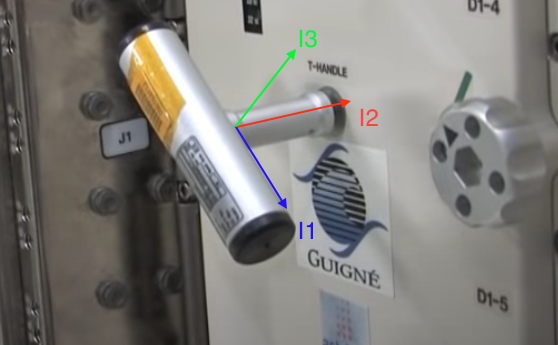
\includegraphics[width=0.5\textwidth]{T_handle_axes.png}
		\caption{The notation adopted for the three moments of inertia shown on top of the T-handle. $I_1$ is the smallest moment of inertia while $I_3$ is the largest.}\label{T_handle_axes}
	\end{figure}
	
	\noindent \textbf{Note:} I don't claim that the results above are very accurate, they are order of magnitude estimates based on sizes I can judge from the screen.
	I am confident that a much better estimation can be extracted with some more effort and by computing the moment of inertia tensor directly through a CAD model.

	The \textbf{Results} folder has several .gifs generated using these numbers and initial values in the range 0.1 -- 1 Hz along the intermediate axis with a perturbation which is 100 times smaller about the smallest moment of inertia.
	These indeed appear quite close to what is seen on the video, but just for each case, I will compare the numerical results to the perturbative solution based on \eqref{Perturbed_oscillator} to confirm.

	\subsection{Numerical vs. perturbative results}
	For verification purposes, I want to compare the numerical solution to what is predicted by the linearized equations (for small perturbations).
	Taking the definition \eqref{kappa_eq}, the general solution to the 2nd order linear differential equation \eqref{Perturbed_oscillator} is 
	\begin{eqnarray}\label{dom1_sol_stable}
		\delta \omega_1 = c_1 \cos( \kappa t ) + c_2 \sin( \kappa t ),
	\end{eqnarray} 
	when $I_3$ is the largest or smallest moment of inertia, and 
	\begin{eqnarray}\label{dom1_sol_unstable}
		\delta \omega_1 = c_1 \exp( \kappa t ) + c_2 \exp( \kappa t )
	\end{eqnarray}
	when $I_3$ is the intermediate moment of inertia.
	In either of these equations, the constants $c_1$ and $c_2$ are determined fully by the initial conditions (what $\delta \vec{\omega}(0)$ is).
	One can also integrate \eqref{Perturbed_Euler_2} given the $\delta \omega_1$ solution and obtain the function $\delta \omega_2(t)$ accordingly.
	Focusing on the case where $I_3$ is the largest or smallest moment of inertia, this gives 
	\begin{eqnarray}\label{dom2_sol_stable}
		\delta \omega_2 = \Theta \left[ c_1 \sin( \kappa t ) - c_2 \cos( \kappa t ) \right],
	\end{eqnarray}
	where I have defined an axiluary dimensionless quantity which comes out of the integration as
	\begin{eqnarray}
		\Theta = \sqrt{ \frac{ (I_3 - I_1) I_1 }{ ( I_2 - I_3 ) I_2 } }.
	\end{eqnarray}
	It is simple to see that \eqref{dom1_sol_stable} and \eqref{dom2_sol_stable} along with $\delta \omega_3 = 0$ indeed solve the system of equations \eqref{Perturbed_Euler_1}-\eqref{Perturbed_Euler_3}.
	As expected, the $\delta \vec{\omega}$ vector describes a periodic closed trajectory (ellipse as we'll see bellow) which depends on the initial data when perturbed lightly about the largest or smallest moment of inertia -- it is precession.
	
	Now we can choose a particular starting state to use for verification purposes.
	A simple option is to perturb the angular velocity only in one direction.
	Suppose that the initial perturbation vector is $\delta \vec{\omega}( 0 ) = [ \delta \omega , 0 , 0 ]^T$.
	Then applying the boundary conditions $c_1 = \delta \omega$ and $c_2 = 0$ which leads us to the full angular rate solution (up to $O(\delta \omega^2)$ terms) as
	\begin{eqnarray}\label{Perturbative_result}
		\vec{\omega} = 
		\begin{bmatrix}
				\delta \omega \cos( \kappa t ) \\
				\Theta \delta \omega \sin( \kappa t ) \\
				\Omega
		\end{bmatrix}.
	\end{eqnarray}

	It is now straightforward to check whether this solution matches with our numerical solution.
	The script $\mathrm{Perturbative\_Test.py}$ executes and plots exactly a comparison between the result \eqref{Perturbative_result} and the numerical integration for the same initial conditions $\vec{\omega}( 0 ) = [ \delta \omega , 0 , \Omega ]^T$.
	Figure \ref{Numerical_vs_Perturbative_plot} shows the results for two different ratios of the perturbation to the "primary" angular velocity.

	\begin{figure}[ht]
		\subfloat[$\delta\omega/\Omega = 0.1$]{
			\begin{minipage}[c][1\width]{
				0.5\textwidth}
			 	\centering
			 	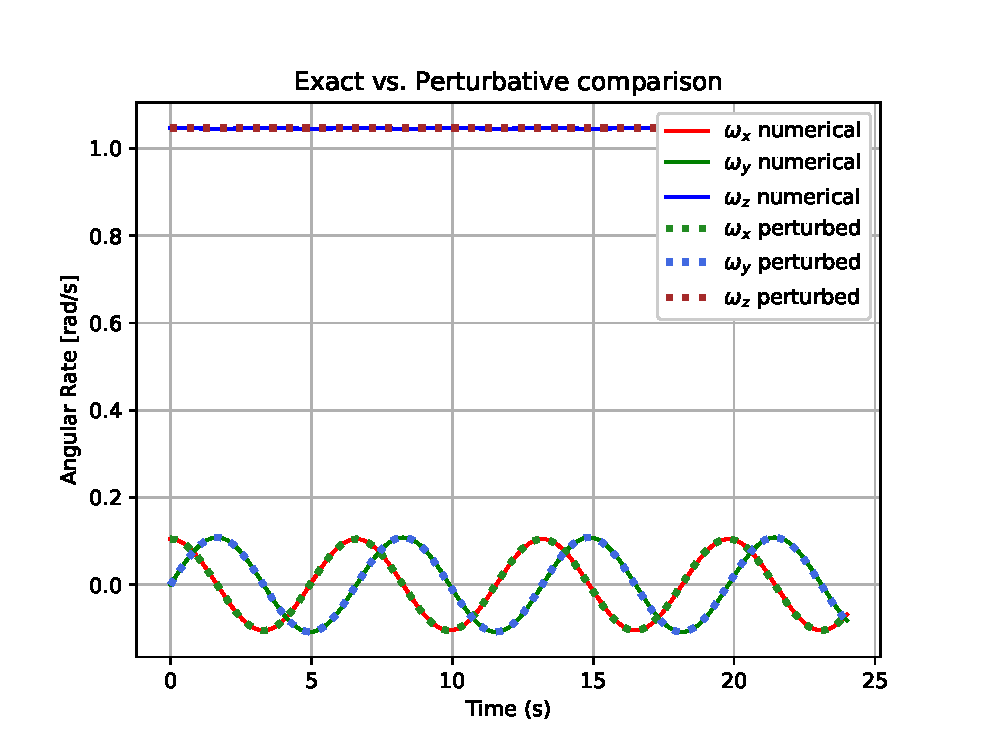
\includegraphics[width=1\textwidth]{Num_vs_Perturbed_Comparison_0.100scale.eps}
		  	\end{minipage}}
		\subfloat[$\delta\omega/\Omega = 0.5$]{
		  	\begin{minipage}[c][1\width]{
				0.5\textwidth}
				\centering
				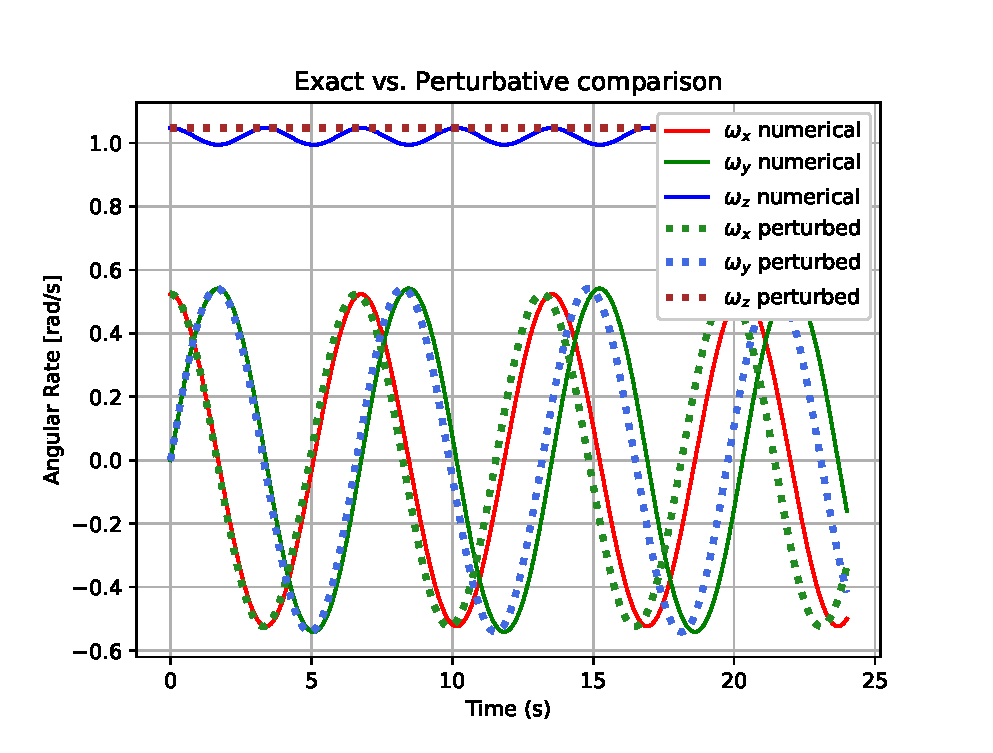
\includegraphics[width=1\textwidth]{Num_vs_Perturbed_Comparison_0.500scale.eps}
		  	\end{minipage}}
	  	\caption{Comparison of the perturbative and numerical solutions for the same body with initial conditions ratio $\delta \omega/\Omega$ equal to 0.1  and 0.5 respectively.}\label{Numerical_vs_Perturbative_plot}
	\end{figure}
	
	It is quite evident that the approximation holds much better in the first case where $O(\delta\omega^2)$ is only a 1\% correction to the end result.
	One can hardly see a deviation between the two results in this case.
	In the latter case, the perturbative solution starts exactly on the numerical one but it diverges much faster since the error $O(\delta \omega^2)$ is about 25\% ($0.5^2$) and higher terms would be needed to retain the accuracy.
	This is well expected and of course the larger the ratio of $\delta \omega/\Omega$ becomes, the faster our approximation will break down.
	
	Nevertheless, it shows that the numerical solver acts just as it should in the "weak regime" of the equations which is often a good test when no exact solution in the full non-linear regime can be obtained.
	One can easily check that similar small deviations with primary $\Omega$ around the smallest moment of inertia (X-axis) will also lead to very good agreement between the perturbative solution and the numerical solver.

	On the other hand, some of you might try to modify the code in order to see how well the approximation works in the case of intermediate axis rotation.
	More generally, you might want to see if you can see the "flip" of the T-handle from the perturbation-only?
	A quick glimpse at \eqref{dom1_sol_unstable} should persuade you that the answer is a "no".
	The two exponentials are completely unconstrained - arbitrarily small perturbation $\delta \omega$ will grow indefinitely which is definitely not a physical behaviour.
	The reason for that is very simple -- the linear equations \eqref{Perturbed_Euler_1}-\eqref{Perturbed_Euler_3} are only an approximation around an equilibrium point.
	If you think about the differential equation as a trajectory in some 3D space (in this case the space would be a hypersphere), linearizing the equations is equivalent to solving them on a hyperplane which is tangent to that space instead of doing so on the real space.
	The linearization "blurs" the curvature of the solution around the equilibrium point.
	Of course, if you stay very close to the point - this is a good approximation (the Earth looks flat up close).
	When the solution is inherently unstable, however (like the intermediate axis case), it moves away from that equilibrium and towards a region where the approximation fails completely.
	This is quite apparent in this case - the real angular velocity of an isolated body cannot change indefinitely (it is bound by the conservation of angular momentum), while the perturbative solution \eqref{dom1_sol_unstable} predicts unbounded growth.
	Geometrically speaking - one is a trajectory on a sphere while the other is its projection on a plane tangent to that sphere (with the pole at infinity)!
	If you are interested in the geometrical description and interpretation of such phenomena, \cite{Geometry_Frankel} is an excellent book with many applications (including rigid body dynamics) to get you started!

	\section{Conclussions}
	I started this small project to explain a phenomenon which I found quite interesting to model as an undergraduate.
	Probably the most interesting thing about the intermediate axis theorem to me was that it is something we can see all around us (even by throwing a textbook) but very few people have an intuition about it even though it was first described some 200 years ago!
	Beyond the phenomenon itself, I hope that you found its description and my rumbling about stability, non-linear systems and geometry useful (or at least interesting)!
	This document and the accompanying code have no purpose beyond education!
	
	\newpage
	\begin{thebibliography}{9}

	\bibitem{David_Tong}
	D.Tong, \textit{Lecture Notes on Classical Dynamics}, available \href{http://www.damtp.cam.ac.uk/user/tong/dynamics/clas.pdf}{here}.

	\bibitem{Goldstein}
	H.~Goldstein, C.~Poole and J.~Safko, \textit{Classical Mechanics}.
	
	\bibitem{ADCS_bible}
	F.~Landis~Markley and John~L.~Crassidis, \textit{Fundamentals of Spacecraft Attitude Determination and Control}.

	\bibitem{Geometry_Frankel}
	T.~Frankel, \textit{The Geometry of Physics: An Introduction}.


	\end{thebibliography}

\end{document}